\documentclass[aspectratio=169]{beamer}
 
\usepackage[utf8]{inputenc}
\usepackage{lipsum}

%%%%%%%%%%%%%%%%%%%%%%%%%%%%%%%%%%%%%%%%%%%%%%%%
% Set Helvetica Font in Text and Math in LaTeX %
%%%%%%%%%%%%%%%%%%%%%%%%%%%%%%%%%%%%%%%%%%%%%%%%
\usepackage[helvet]{sfmath}
\usepackage[scaled=1]{helvet}
\usepackage[T1]{fontenc}
\renewcommand\familydefault{\sfdefault} 
\everymath={\sf}
\usepackage{fontspec}

\usepackage{subcaption}

\hypersetup{
    colorlinks=true,
    linkcolor=blue,
    filecolor=magenta,      
    urlcolor=cyan,
    pdftitle={Overleaf Example},
%    pdfpagemode=FullScreen,
}

% use settings files
\usetheme[progressbar=frametitle]{metropolis}

%%%%%%%%%%%%%%%%%%%%%%%%%%%%%%%%%%%%%%%%%%%%%%%%%%%%%%%%%%%%%%%%
% Color settings
\definecolor{ru_white}{HTML}{FFFFFF}
\definecolor{ru_red}{HTML}{ed1c24}
\definecolor{black}{HTML}{000000}
\definecolor{gray}{HTML}{A9A9A9}
\definecolor{light_gray}{HTML}{E0E0E0}
\setbeamercolor{frametitle}
{
  use=palette primary,
  parent=palette primary,
  fg = ru_white,
  bg = ru_red
}
% fg means "foreground" and bg means "background"
\setbeamercolor{title separator}{ fg=ru_red }
\setbeamercolor{section bar}{ fg=ru_red, bg=ru_red }
\setbeamercolor{progress bar in section page}{
%   use=progress bar,
%   parent=progress bar
    fg=black,
    bg=ru_red
}

\setbeamercolor{normal text}{%
  fg=black,
  bg=white
}
\setbeamercolor{alerted text}{%
  fg=ru_red,
}
\setbeamercolor{example text}{%
  fg=black,
}

\setbeamercolor{progress bar in head/foot}{ fg=black, bg=gray } % use this line to enable the progress bar
% \setbeamercolor{progress bar in head/foot}{ fg=black, bg=black } % use this line to have a divider instead of a progress bar

% \setbeamertemplate{frame numbering}{} % uncomment this line to remove slide numbers
\titlegraphic{\hfill
\includegraphics[height=2.0cm]{images/HR_logo_hringur_hires}}
%\logo{
\includegraphics[width=.1\textwidth]{images/HR_logo_hringur_lowres}\vspace{-0.05\paperwidth}\hspace*{.04\paperwidth}} % uncomment this line to include the RU logo on each slide
\logo{
\includegraphics[width=.1\textwidth]{images/HR_logo_hringur_lowres}\vspace{-0.05\paperwidth}\hspace*{0.5\paperwidth}} % uncomment this line to include the RU logo on each slide

\setbeamertemplate{itemize items}[default]

\setbeamerfont{bibliography entry author}{size=\tiny,series=\normalfont}
\setbeamerfont{bibliography entry title}{size=\tiny,series=\bfseries}
\setbeamerfont{bibliography entry location}{size=\tiny,series=\normalfont}
\setbeamerfont{bibliography entry note}{size=\tiny,series=\normalfont}

\makeatletter
\setlength{\metropolis@progressinheadfoot@linewidth}{1pt}               % thickness of progress bar on normal pages
\setlength{\metropolis@titleseparator@linewidth}{0.5pt}                 % thickness of separator on title page
\setlength{\metropolis@progressonsectionpage@linewidth}{0.5pt}          % thickness of progress bar on section page


\setbeamertemplate{frametitle}{%
    \vspace*{-0.12cm}
     \begin{beamercolorbox}[wd=\paperwidth,ht=2ex,dp=0.8ex,left]{frametitle}%
    %   \hspace*{2ex}\insertframetitle%
        % \vspace*{\fill}
        \hspace*{2ex}\insertframetitle%
        % \vspace*{\fill}
     \end{beamercolorbox}}

\usepackage{ifxetex,ifluatex}

\usepackage{tikz}
\usepackage{framed}

% conditional for xetex or luatex
% \newif\ifxetexorluatex
% \ifxetex
%   \xetexorluatextrue
% \else
%   \ifluatex
%     \xetexorluatextrue
%   \else
%     \xetexorluatexfalse
%   \fi
% \fi

% \ifxetexorluatex
%   \usepackage{libertine} % or use \setmainfont to choose any font on your system
%   \newfontfamily[Ligatures=TeX]{Linux Libertine O} % selects Libertine as the quote font
% \else
%   \usepackage{libertine} % or any other font package
%   \newcommand* {\fontfamily{LinuxLibertineT-LF}} % selects Libertine as the quote font
% \fi

\newcommand*\quotesize{60} % if quote size changes, need a way to make shifts relative
% Make commands for the quotes
\newcommand*{\openquote}
   {\tikz[remember picture,overlay,xshift=-4ex,yshift=-2.5ex]
   \node (OQ) { \fontsize{\quotesize}{\quotesize}\selectfont``};\kern0pt}

\newcommand*{\closequote}[1]
  {\tikz[remember picture,overlay,xshift=4ex,yshift={#1}]
   \node (CQ) { \fontsize{\quotesize}{\quotesize}\selectfont''};}

% select a colour for the shading
\definecolor{shade_color}{HTML}{F8F8F8}
\colorlet{shadecolor}{light_gray}

\newcommand*\shadedauthorformat{\emph} % define format for the author argument

% Now a command to allow left, right and centre alignment of the author
\newcommand*\authoralign[1]{%
  \if#1l
    \def\authorfill{}\def\quotefill{\hfill}
  \else
    \if#1r
      \def\authorfill{\hfill}\def\quotefill{}
    \else
      \if#1c
        \gdef\authorfill{\hfill}\def\quotefill{\hfill}
      \else\typeout{Invalid option}
      \fi
    \fi
  \fi}
% wrap everything in its own environment which takes one argument (author) and one optional argument
% specifying the alignment [l, r or c]
%
\newenvironment{shadequote}[2][l]%
{\authoralign{#1}
\ifblank{#2}
   {\def\shadequoteauthor{}\def\yshift{-2ex}\def\quotefill{\hfill}}
   {\def\shadequoteauthor{\par\authorfill\shadedauthorformat{#2}}\def\yshift{2ex}}
\begin{snugshade}\begin{quote}\openquote}
{\shadequoteauthor\quotefill\closequote{\yshift}\end{quote}\end{snugshade}}

% Other packages
\usepackage{enumitem}
\setitemize{label=\usebeamerfont*{itemize item}%
  \usebeamercolor[fg]{itemize item}
  \usebeamertemplate{itemize item}}

\usepackage{amssymb}
\newcommand*{\QEDA}{\hfill\ensuremath{\blacksquare}}

\usepackage{datetime}
\newdateformat{specialdate}{\twodigit{\THEDAY} \ \monthname[\THEMONTH] \THEYEAR}
%%%%%%%%%%%%%%%%%%%%%%%%%%%%%%%%%%%%%%%%%%%%%%%%%%%%%%%%%%%%%%%%%

\newcommand{\nologo}{\setbeamertemplate{logo}{}}
\newcommand{\yeslogo}{\logo{\vspace{-0.5cm}
\includegraphics[width=1.5cm]{./images/HR_logo_hringur_lowres}\hspace{0.5cm}}}

\yeslogo

\newif\ifpause
%\pausetrue
\pausefalse
\newcommand{\mypause}{\ifpause \pause \fi}

%Information to be included in the title page:
\title{Autonomous Drone Landing with Fiducial Markers\\and a Gimbal-Mounted Camera for Active Tracking}
\author{Joshua Springer}
\institute{Reykjavik University\\Department of Computer Science}

\date{\specialdate\today}

\begin{document}

\maketitle

\nologo

\begin{frame}{Fiducial Markers}
	\vspace*{\fill}
	\begin{figure}[]
	    \centering
	    \begin{subfigure}[b]{0.2\linewidth}
		
\includegraphics[width=\textwidth]{./images/tagCustom48h12_00002_00001_00000}
		\caption{April Tag 48h12}
		\label{figure:apriltag48h12}
	    \end{subfigure}
		\hspace{0.05\linewidth}
	    \begin{subfigure}[b]{0.2\linewidth}
		\includegraphics[width=\textwidth]{./images/tagCustom24h10_00002_00001_00000}
		\caption{April Tag 24h10}
		\label{figure:apriltag24h10}
	    \end{subfigure}
		\hspace{0.05\linewidth}
	    \begin{subfigure}[b]{0.2\linewidth}
		
\includegraphics[width=\textwidth]{./images/whycode_20_8}
		\caption{WhyCode (Orig)}
		\label{figure:whycode_single}
	    \end{subfigure}
		\hspace{0.05\linewidth}
	    \begin{subfigure}[b]{0.2\linewidth}
		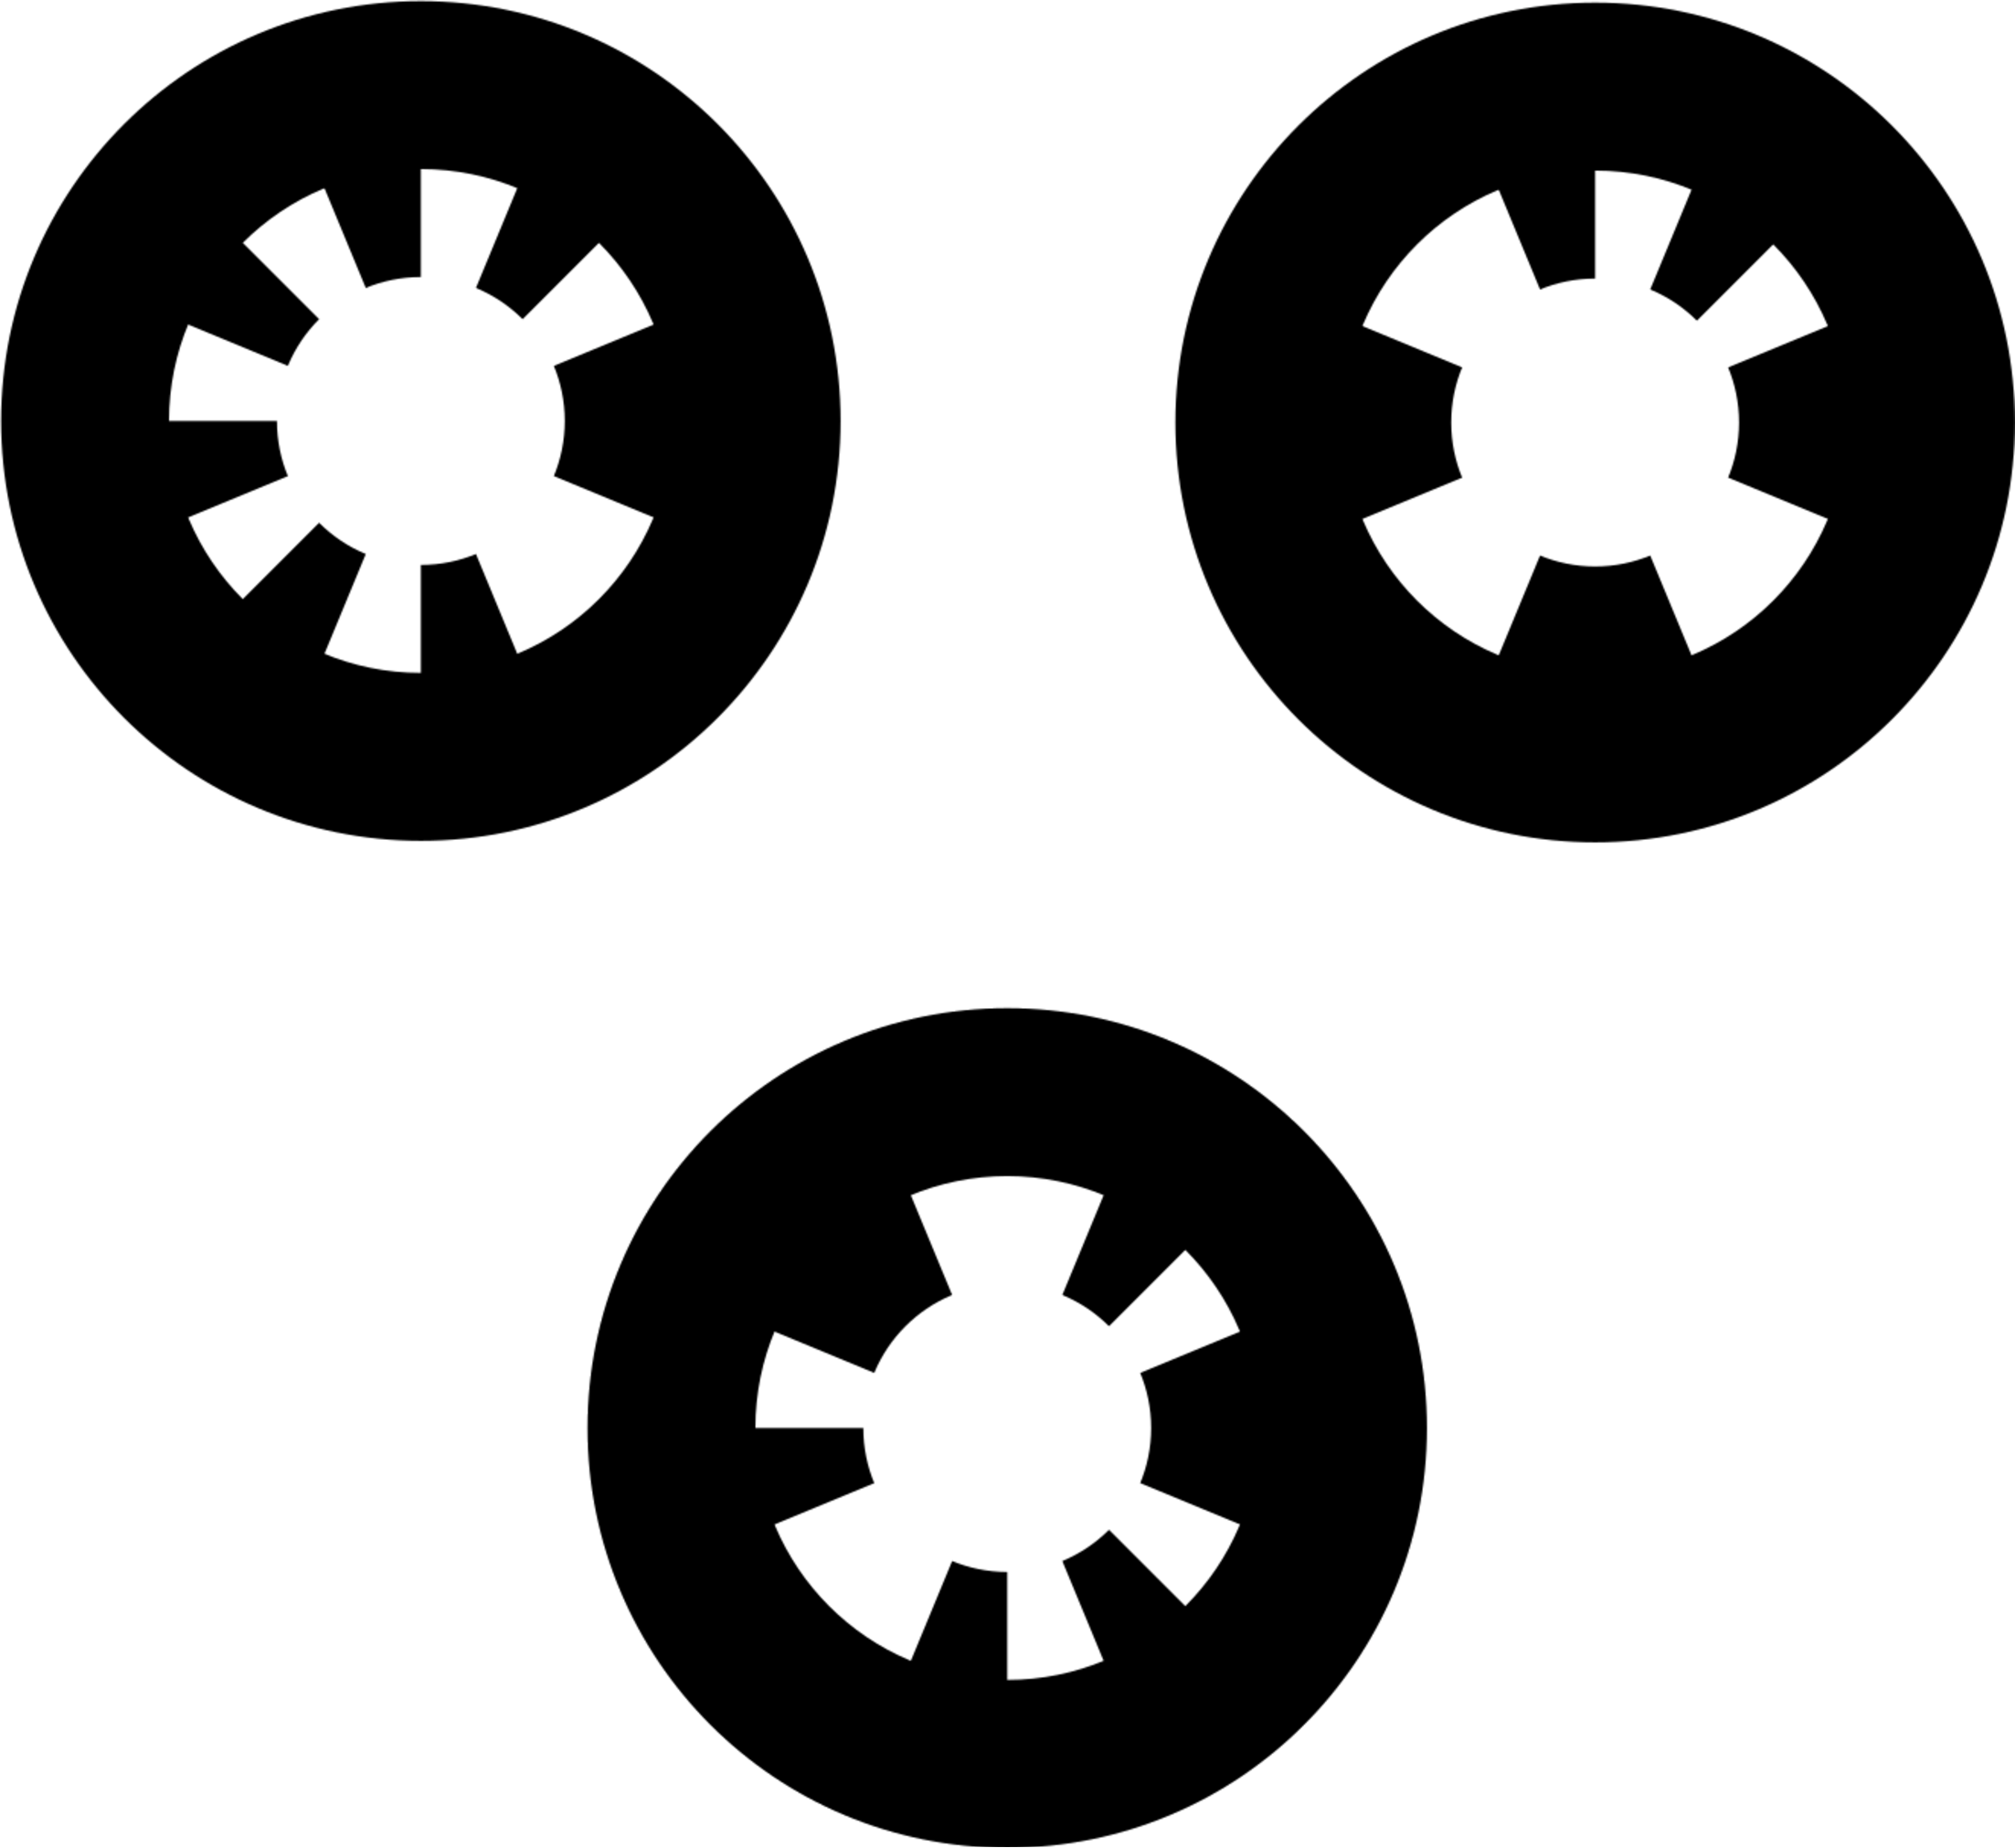
\includegraphics[width=\textwidth]{./images/whycode_multi}
		\caption{WhyCode Multi}
		\label{figure:whycode_bundle}
	    \end{subfigure}
	    \label{figure:marker_setup}
	\end{figure}
	\vspace*{\fill}
\end{frame}

\begin{frame}{Orientation Ambiguity}
	\begin{itemize}
		\item Marker \emph{position} $\rightarrow$ accurate
		\item Marker \emph{orientation} $\rightarrow$ ambiguous
	\end{itemize}
\end{frame}

\begin{frame}{The Downward-facing Camera Axiom}
\end{frame}

\begin{frame}{Testing Platform: DJI Spark}
	\begin{columns}
	\begin{column}{0.5\textwidth}
	\begin{itemize}
		\item Small quadcopter
		\item Gimbal-mounted camera
		\item DJI Mobile SDK
	\end{itemize}
	\end{column}
	\begin{column}{0.5\textwidth}
		\centering
		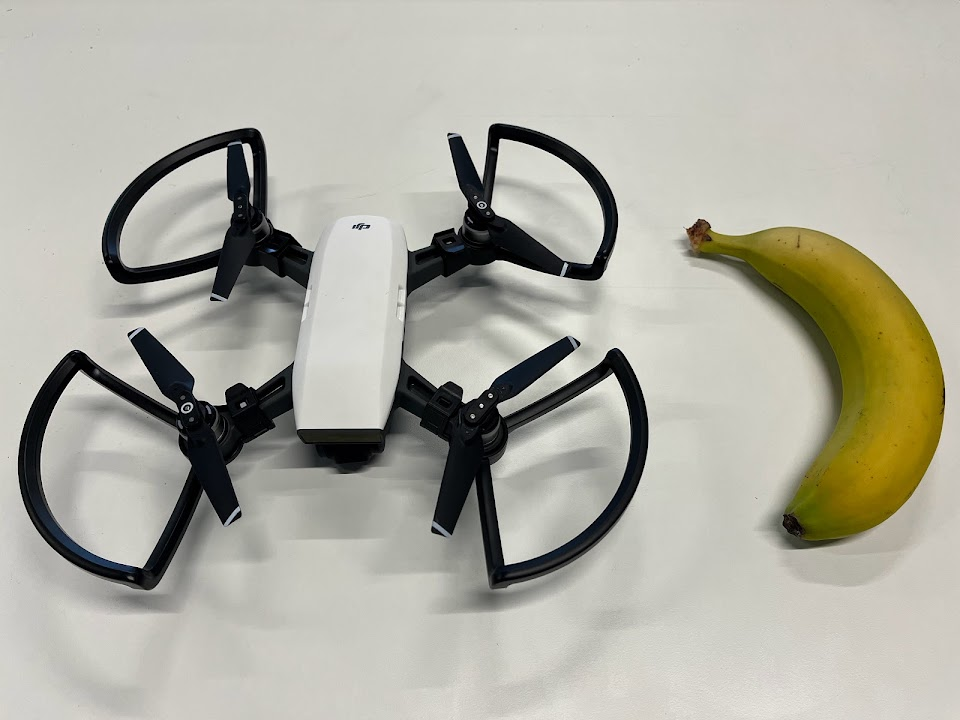
\includegraphics[width=\textwidth]{./images/dji_spark}
	\end{column}
	\end{columns}
\end{frame}

\begin{frame}{Testing Platform: Software Side}
	\begin{columns}
	\begin{column}{0.5\textwidth}
	\begin{itemize}
		\item DJI Mobile SDK: App-style artchitecture
		\item Export video to Raspberry Pi 4 companion board
		\item Return control signals
	\end{itemize}
	\end{column}
	\begin{column}{0.5\textwidth}
		\centering
		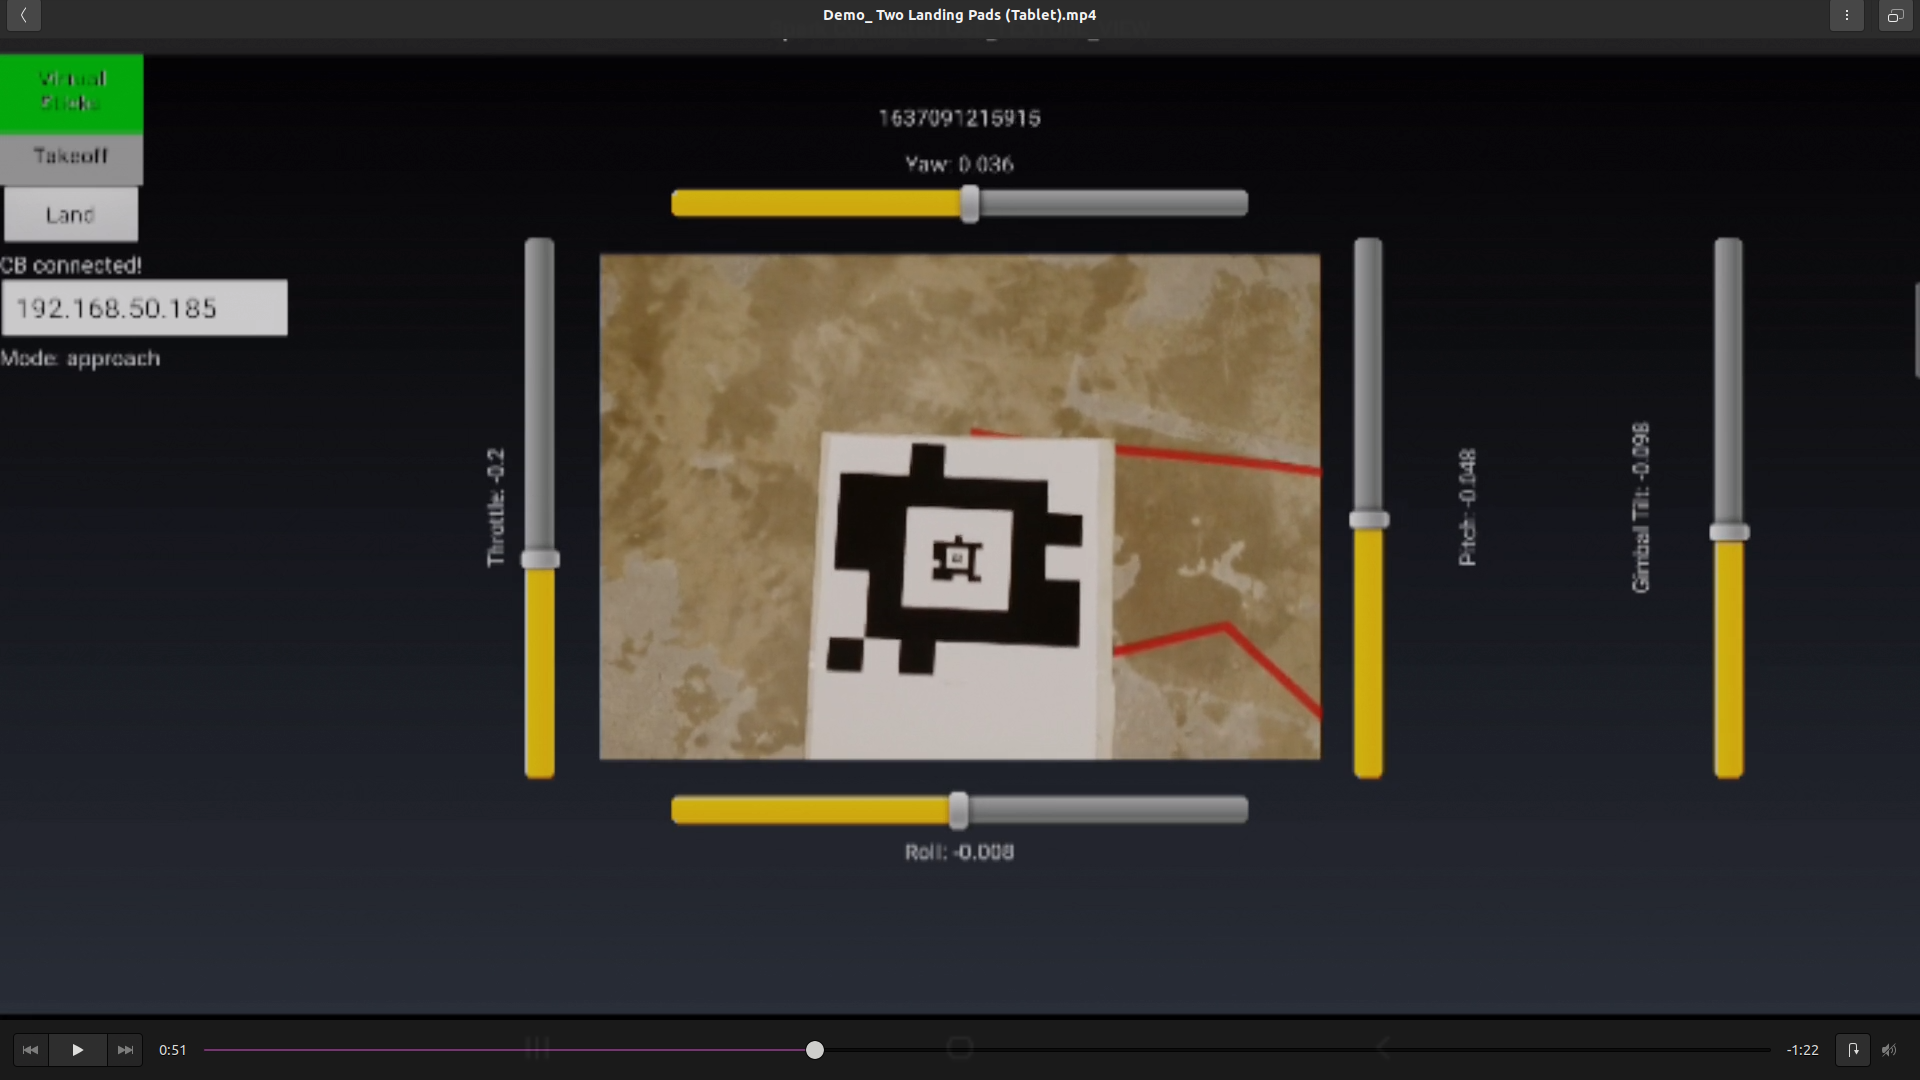
\includegraphics[width=\textwidth]{./images/tablet_screenshot}
	\end{column}
	\end{columns}
\end{frame}

\begin{frame}{Example Tracking Performance}
\end{frame}

\begin{frame}{Example Landing Trajectory}
\end{frame}

\begin{frame}{Example Control Outputs}
\end{frame}

\begin{frame}{Erroneous Control Outputs}
\end{frame}

\begin{frame}{Erroneous Landing Trajectory}
\end{frame}

\begin{frame}{Landing Radii}
\end{frame}

\begin{frame}{Future Work}
	\begin{itemize}
		\item Use another drone platform
		\begin{itemize}
			\item Phantom, Mavic
			\item More gimbal tilt range
		\end{itemize}
		\item Connect companion board directly to controller
		\item Test 3 separate methods for each fiducial system:
		\begin{itemize}
			\item Raw/unfiltered marker pose
			\item Filtered marker pose, e.g.~KF
			\item Marker \emph{position} and gimbal \emph{orientation} for pose transforms
		\end{itemize}
	\end{itemize}
\end{frame}

\begin{frame}{Main Messages}
	\begin{itemize}
		\item \emph{Actuated}, gimbal-mounted camera
			\mypause $\rightarrow$ easier to search for the landing pad.
		\mypause\item Orientation ambiguity, discontinuities
			\mypause $\rightarrow$ pose estimation is harder.
		\mypause\item Autonomous precision landing still possible
			\mypause but can be improved.
	\end{itemize}
\end{frame}


%\begin{frame}{}
%\end{frame}

\end{document}
